\ifx\allfiles\undefined
\documentclass[12pt, a4paper, oneside, UTF8]{ctexbook}
\def\path{../config}
\usepackage{amsmath}
\usepackage{amsthm}
\usepackage{array}
\usepackage{amssymb}
\usepackage{graphicx}
\usepackage{mathrsfs}
\usepackage{enumitem}
\usepackage{geometry}
\usepackage[colorlinks, linkcolor=black]{hyperref}
\usepackage{stackengine}
\usepackage{yhmath}
\usepackage{extarrows}
% \usepackage{unicode-math}
\usepackage{esint}
\usepackage{multirow}
\usepackage{fancyhdr}
\usepackage[dvipsnames, svgnames]{xcolor}
\usepackage{listings}
\usepackage{float} % Required for the H float option
\definecolor{mygreen}{rgb}{0,0.6,0}
\definecolor{mygray}{rgb}{0.5,0.5,0.5}
\definecolor{mymauve}{rgb}{0.58,0,0.82}
\definecolor{NavyBlue}{RGB}{0,0,128}
\definecolor{Rhodamine}{RGB}{255,0,255}
\definecolor{PineGreen}{RGB}{0,128,0}

\graphicspath{ {figures/},{../figures/}, {config/}, {../config/} }

\linespread{1.6}

\geometry{
    top=25.4mm, 
    bottom=25.4mm, 
    left=20mm, 
    right=20mm, 
    headheight=2.17cm, 
    headsep=4mm, 
    footskip=12mm
}

\setenumerate[1]{itemsep=5pt,partopsep=0pt,parsep=\parskip,topsep=5pt}
\setitemize[1]{itemsep=5pt,partopsep=0pt,parsep=\parskip,topsep=5pt}
\setdescription{itemsep=5pt,partopsep=0pt,parsep=\parskip,topsep=5pt}

\lstset{
    language=Mathematica,
    basicstyle=\tt,
    breaklines=true,
    keywordstyle=\bfseries\color{NavyBlue}, 
    emphstyle=\bfseries\color{Rhodamine},
    commentstyle=\itshape\color{black!50!white}, 
    stringstyle=\bfseries\color{PineGreen!90!black},
    columns=flexible,
    numbers=left,
    numberstyle=\footnotesize,
    frame=tb,
    breakatwhitespace=false,
} 

\lstset{
    language=TeX, % 设置语言为 TeX
    basicstyle=\ttfamily, % 使用等宽字体
    breaklines=true, % 自动换行
    keywordstyle=\bfseries\color{NavyBlue}, % 关键字样式
    emphstyle=\bfseries\color{Rhodamine}, % 强调样式
    commentstyle=\itshape\color{black!50!white}, % 注释样式
    stringstyle=\bfseries\color{PineGreen!90!black}, % 字符串样式
    columns=flexible, % 列的灵活性
    numbers=left, % 行号在左侧
    numberstyle=\footnotesize, % 行号字体大小
    frame=tb, % 顶部和底部边框
    breakatwhitespace=false % 不在空白处断行
}

% \begin{lstlisting}[language=TeX] ... \end{lstlisting}

% 定理环境设置
\usepackage[strict]{changepage} 
\usepackage{framed}

\definecolor{greenshade}{rgb}{0.90,1,0.92}
\definecolor{redshade}{rgb}{1.00,0.88,0.88}
\definecolor{brownshade}{rgb}{0.99,0.95,0.9}
\definecolor{lilacshade}{rgb}{0.95,0.93,0.98}
\definecolor{orangeshade}{rgb}{1.00,0.88,0.82}
\definecolor{lightblueshade}{rgb}{0.8,0.92,1}
\definecolor{purple}{rgb}{0.81,0.85,1}

\theoremstyle{definition}
\newtheorem{myDefn}{\indent Definition}[section]
\newtheorem{myLemma}{\indent Lemma}[section]
\newtheorem{myThm}[myLemma]{\indent Theorem}
\newtheorem{myCorollary}[myLemma]{\indent Corollary}
\newtheorem{myCriterion}[myLemma]{\indent Criterion}
\newtheorem*{myRemark}{\indent Remark}
\newtheorem{myProposition}{\indent Proposition}[section]

\newenvironment{formal}[2][]{%
	\def\FrameCommand{%
		\hspace{1pt}%
		{\color{#1}\vrule width 2pt}%
		{\color{#2}\vrule width 4pt}%
		\colorbox{#2}%
	}%
	\MakeFramed{\advance\hsize-\width\FrameRestore}%
	\noindent\hspace{-4.55pt}%
	\begin{adjustwidth}{}{7pt}\vspace{2pt}\vspace{2pt}}{%
		\vspace{2pt}\end{adjustwidth}\endMakeFramed%
}

\newenvironment{definition}{\vspace{-\baselineskip * 2 / 3}%
	\begin{formal}[Green]{greenshade}\vspace{-\baselineskip * 4 / 5}\begin{myDefn}}
	{\end{myDefn}\end{formal}\vspace{-\baselineskip * 2 / 3}}

\newenvironment{theorem}{\vspace{-\baselineskip * 2 / 3}%
	\begin{formal}[LightSkyBlue]{lightblueshade}\vspace{-\baselineskip * 4 / 5}\begin{myThm}}%
	{\end{myThm}\end{formal}\vspace{-\baselineskip * 2 / 3}}

\newenvironment{lemma}{\vspace{-\baselineskip * 2 / 3}%
	\begin{formal}[Plum]{lilacshade}\vspace{-\baselineskip * 4 / 5}\begin{myLemma}}%
	{\end{myLemma}\end{formal}\vspace{-\baselineskip * 2 / 3}}

\newenvironment{corollary}{\vspace{-\baselineskip * 2 / 3}%
	\begin{formal}[BurlyWood]{brownshade}\vspace{-\baselineskip * 4 / 5}\begin{myCorollary}}%
	{\end{myCorollary}\end{formal}\vspace{-\baselineskip * 2 / 3}}

\newenvironment{criterion}{\vspace{-\baselineskip * 2 / 3}%
	\begin{formal}[DarkOrange]{orangeshade}\vspace{-\baselineskip * 4 / 5}\begin{myCriterion}}%
	{\end{myCriterion}\end{formal}\vspace{-\baselineskip * 2 / 3}}
	

\newenvironment{remark}{\vspace{-\baselineskip * 2 / 3}%
	\begin{formal}[LightCoral]{redshade}\vspace{-\baselineskip * 4 / 5}\begin{myRemark}}%
	{\end{myRemark}\end{formal}\vspace{-\baselineskip * 2 / 3}}

\newenvironment{proposition}{\vspace{-\baselineskip * 2 / 3}%
	\begin{formal}[RoyalPurple]{purple}\vspace{-\baselineskip * 4 / 5}\begin{myProposition}}%
	{\end{myProposition}\end{formal}\vspace{-\baselineskip * 2 / 3}}


\newtheorem{example}{\indent \color{SeaGreen}{Example}}[section]
\renewcommand{\proofname}{\indent\textbf{\textcolor{TealBlue}{Proof}}}
\newenvironment{solution}{\begin{proof}[\indent\textbf{\textcolor{TealBlue}{Solution}}]}{\end{proof}}

% 自定义命令的文件

\def\d{\mathrm{d}}
\def\R{\mathbb{R}}
%\newcommand{\bs}[1]{\boldsymbol{#1}}
%\newcommand{\ora}[1]{\overrightarrow{#1}}
\newcommand{\myspace}[1]{\par\vspace{#1\baselineskip}}
\newcommand{\xrowht}[2][0]{\addstackgap[.5\dimexpr#2\relax]{\vphantom{#1}}}
\newenvironment{mycases}[1][1]{\linespread{#1} \selectfont \begin{cases}}{\end{cases}}
\newenvironment{myvmatrix}[1][1]{\linespread{#1} \selectfont \begin{vmatrix}}{\end{vmatrix}}
\newcommand{\tabincell}[2]{\begin{tabular}{@{}#1@{}}#2\end{tabular}}
\newcommand{\pll}{\kern 0.56em/\kern -0.8em /\kern 0.56em}
\newcommand{\dive}[1][F]{\mathrm{div}\;\boldsymbol{#1}}
\newcommand{\rotn}[1][A]{\mathrm{rot}\;\boldsymbol{#1}}

% 修改参数改变封面样式,0 默认原始封面、内置其他1、2、3种封面样式
\def\myIndex{0}


\ifnum\myIndex>0
    \input{\path/cover_package_\myIndex}
\fi

\def\myTitle{标题:一份LaTeX笔记模板}
\def\myAuthor{作者名称}
\def\myDateCover{封面日期: \today}
\def\myDateForeword{前言页显示日期: \today}
\def\myForeword{前言标题}
\def\myForewordText{
    
    这是一个基于\LaTeX{}的模板,用于撰写学习笔记。

    模板旨在提供一个简单、易用的框架,以便你能够专注于内容,而不是排版细节,如不是专业者,不建议使用者在模板细节上花费太多时间,而是直接使用模板进行笔记撰写。遇到问题,再进行调整解决。
}
\def\mySubheading{副标题}


\begin{document}
% \input{\path/cover_text_\myIndex.tex}

\newpage
\thispagestyle{empty}
\begin{center}
    \Huge\textbf{\myForeword}
\end{center}
\myForewordText
\begin{flushright}
    \begin{tabular}{c}
        \myDateForeword
    \end{tabular}
\end{flushright}

\newpage
\pagestyle{plain}
\setcounter{page}{1}
\pagenumbering{Roman}
\tableofcontents

\newpage
\pagenumbering{arabic}
\setcounter{chapter}{-1}
\setcounter{page}{1}

\pagestyle{fancy}
\fancyfoot[C]{\thepage}
\renewcommand{\headrulewidth}{0.4pt}
\renewcommand{\footrulewidth}{0pt}








\else
\fi

\chapter{计算题\&易错题}

\begin{example}
    地震也属于荷载。

    \textbf{错},地震属于作用,不属于荷载。荷载是指作用在结构上的力或力矩,而地震作用是指地震引起的结构响应。{\color{red}{换句话说,狭义上,荷载必须是直接作用。}}

    小技巧,看到带"力"的,比如说惯性力,那必然是直接作用,也就是荷载。
\end{example}

\begin{example}
    当年最大雪深出现时,对应的雪重度一定是本年的最大值.

    \textbf{错},因为雪存在压实的现象,正如第一章里面提到的,雪压力大小$p=\gamma s = \rho g s$,压实状态和反复冻融的雪重度更大,不能一概而论
\end{example}

\begin{example}
    基本雪压是使用期内最大值还是平均值?

    根据荷载的定义,基本雪压是长周期内的最大值,比如在100重现期内的最大值被定义为基本雪压。

    实际上,荷载的定义是基于概率的,荷载的计算是基于统计学的。比如准永久值、频遇值和标准值,这里标准值的重现期最长,理所当然的标准值是最大的。

\end{example}

\begin{example}
    杭州市某拱形屋面建筑,拱高\(f=5m\),拱跨\(l=20m\),求该屋面的雪荷载标准值。

    标准值如果可以直接测量最好,不能就用基本雪压进行推算:
    \[
    s_k = \mu_r s_0
    \]
    查荷载规范附录E,杭州市地面基本雪压:
    \[
    s_0 = 0.45\,\mathrm{kN/m}^2
    \]
    屋面积雪分布系数:
    \[
    \mu_r = \frac{l}{8f} = \frac{20}{8 \times 5} = 0.5
    \]
    符合 \(0.4 \leq \mu_r \leq 1.0\)。
    该屋面雪荷载标准值:
    \[
    s_k = \mu_r s_0 = 0.5 \times 0.45 = 0.225\,\mathrm{kN/m}^2
    \]
\end{example}

\begin{example}
    说明车辆荷载与车道荷载的区别。

车辆荷载:考虑车的尺寸及车的排列方式,以集中荷载的形式作用于车轴(即车轮)位置。

车道荷载:一个虚拟荷载,不考虑车的尺寸及排列方式,将其等效为均布荷载和一个可作用于任意位置的集中荷载形式。对于不同类型的荷载(比如力和力矩),均布荷载和集
中荷载的加载位置通常是不同的,大小也很可能不同。

这时,为了考虑最坏的情况,我们考虑辅助线来施加荷载(比如对于一个简支梁,有一部分加了力,可以让某点弯曲力矩变大,但是加在别的部位反而可能让力矩变小,我们必须考虑最坏的情况,以提高鲁棒性)
\end{example}

\begin{definition}
    准永久值$<$频遇值$<$标准值
\end{definition}

\begin{example}
    什么是土的侧压力?其大小与分布规律与哪些因素有关?

侧压力:挡土墙后的填土因自重或外荷载作用对墙背产生的土压力。

影响因素:墙体可能的移动方向、墙后填土的性质、填土面的形状、墙的截面刚度、地基的变形。
\end{example}

\begin{example}
    已知某挡土墙高 \( H = 9\,\mathrm{m} \),墙背竖直、光滑,填土表面水平。墙后填土为无黏性中砂,重度 \( \gamma = 18\,\mathrm{kN/m}^3 \),内摩擦角 \( \varphi = 30^\circ \)。求作用在挡土墙上的主动土压力 \( E_a \) 与被动土压力 \( E_p \)。

    \begin{align*}
        K_a &= \tan^2\left(45^\circ - \frac{\varphi}{2}\right) = \tan^2(30^\circ) = (0.577)^2 = 0.333 \\
        K_p &= \tan^2\left(45^\circ + \frac{\varphi}{2}\right) = \tan^2(60^\circ) = (1.732)^2 = 3.0 \\
        E_a &= \frac{1}{2} K_a \gamma H^2 = \frac{1}{2} \times 0.333 \times 18 \times 9^2 = 243\,\mathrm{kN/m} \\
        E_p &= \frac{1}{2} K_p \gamma H^2 = \frac{1}{2} \times 3.0 \times 18 \times 9^2 = 2,\!187\,\mathrm{kN/m}
    \end{align*}

    这题的压力计算参考了流体静压的计算,建议画个三角形,同时提醒下,压心是在距底端 \(\frac{H}{3}\) 的位置。

    我们给出朗肯土压力假设下的推导:
    \begin{enumerate}
        \item   土体为半空间弹性体 (竖向压力与深度成正比)
        \item 挡土墙墙背竖直光滑(墙背与填土间无剪应力,墙背为主应力面)
        \item 填土面水平,无超载。
    \end{enumerate}

    摩擦角是一个描述土体临界状态时的参数,这里我们给出刻画土体的摩擦角的定义:
\[
\tau = c + \sigma \tan \varphi
\]
\begin{itemize}
    \item \(c\) 是黏聚力(粘土类土壤的特性)
    \item \(\sigma\) 是法向应力(压在颗粒上的压力)
    \item \(\varphi\) 就是摩擦角,影响剪切强度中的摩擦部分。
\end{itemize}

你可以直观的理解下,这是一个刻画土壤粘聚性的参数,一定的压应力下,如果摩擦角越大,对应的切应力越大,越难以平衡。
因此,摩擦角越大,土壤稳定性越差。显然,当土体的莫尔圆和摩擦角对应的函数相切,这是一个稳定的状态,不论什么时候都不会发生状态的改变。

\begin{figure}[H]
    \centering
    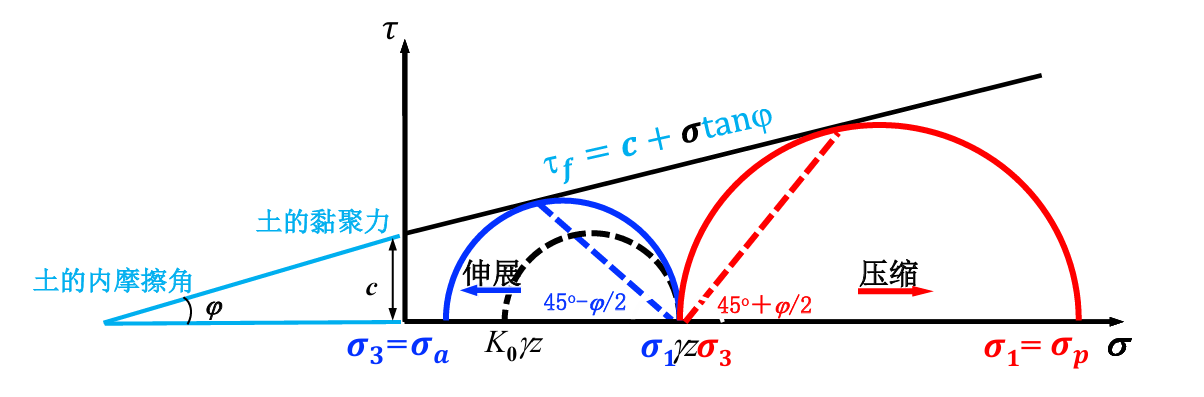
\includegraphics[width=0.7\textwidth]{../figure/2.png}
    \caption{冻胀力作用示意图}
\end{figure}

由材料力学的知识,我们知道这里我们只需要考虑平面应力状态就行了,因为第三个方向没有外加作用力。

按照压应力的大小变化,我们分为主动土压力和被动土压力,其中主动土压力的莫尔圆时刻处于静止土压力的左端,被动土压力处处相反。‘

因为被动土压力是外界荷载持续施加力,我们需要知道这个最大的荷载可以加到什么程度,导致开始滑移,这就是被动土压力的由来。

之后就是三角函数的死算了,没啥意思:

根据莫尔圆和破坏角度的几何关系,有:

\[
\sigma_1 = \sigma_3 \frac{1 + \sin \varphi}{1 - \sin \varphi} + \frac{2 c \sqrt{\sin \varphi}}{1 - \sin \varphi}
\]

其中,

- 当\(\sigma_1\)为垂直主应力,\(\sigma_3\)为水平主应力时,得到\textbf{主动土压力}:
\[
K_a = \frac{\sigma_3}{\sigma_1} = \tan^2 \left(45^\circ - \frac{\varphi}{2}\right) = \frac{1 - \sin \varphi}{1 + \sin \varphi}
\]
- 当\(\sigma_3\)为垂直主应力,\(\sigma_1\)为水平主应力时,得到\textbf{被动土压力}:
\[
K_p = \frac{\sigma_1}{\sigma_3} = \tan^2 \left(45^\circ + \frac{\varphi}{2}\right) = \frac{1 + \sin \varphi}{1 - \sin \varphi}
\]
主动土压力为:
\[
\sigma_a = K_a \gamma z - 2 c \sqrt{K_a}
\]
当土为无黏性土(\(c=0\))时,简化为:
\[
\sigma_a = K_a \gamma z
\]
被动土压力为:
\[
\sigma_p = K_p \gamma z + 2 c \sqrt{K_p}
\]
当土为无黏性土时,简化为:
\[
\sigma_p = K_p \gamma z
\]

\begin{remark}
    这里没提到为什么假设粘性土的应力表现为一个线性的形式,这是朗肯土压力理论的基础假设内容,我也不知道为啥,所以请死记硬背住粘性土的等效高度。
\end{remark}

\begin{figure}[H]
    \centering
    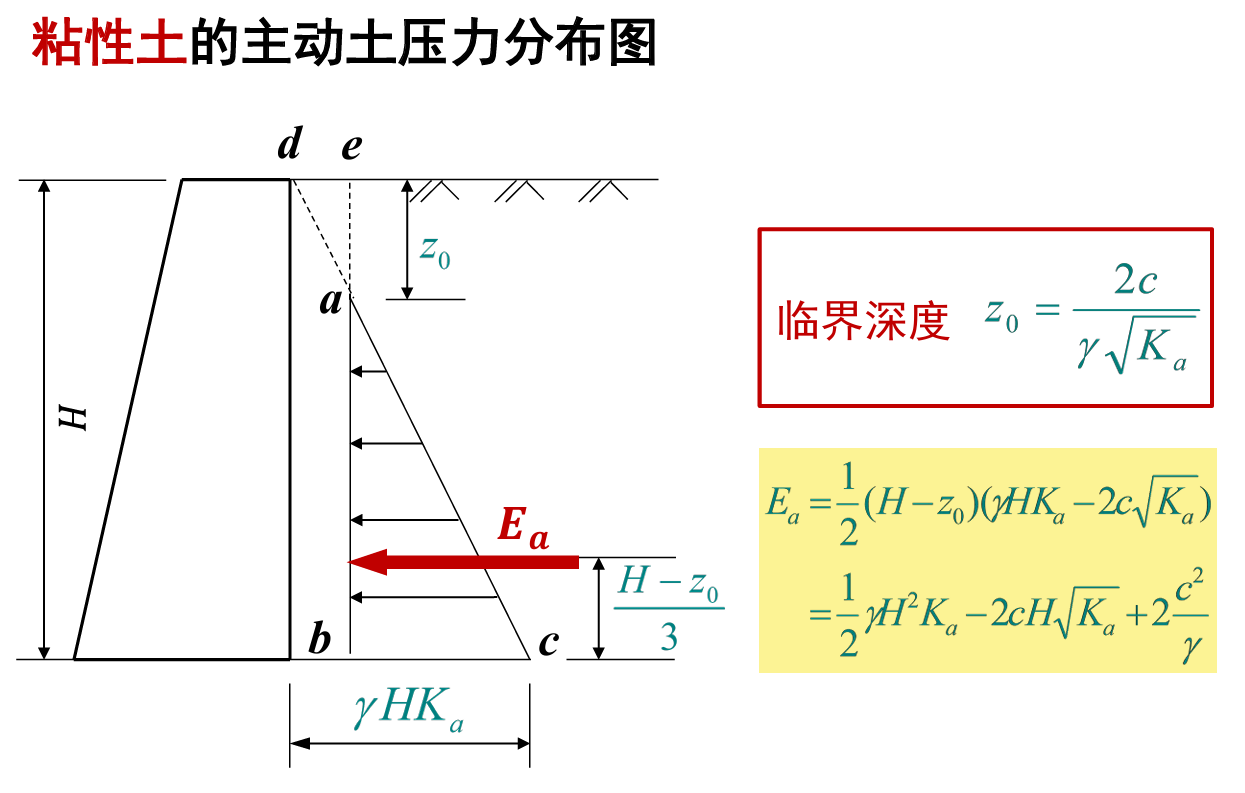
\includegraphics[width=0.8\textwidth]{../figure/zhudong.png}
    \caption{主动土压力}
\end{figure}

\begin{figure}[H]
    \centering
    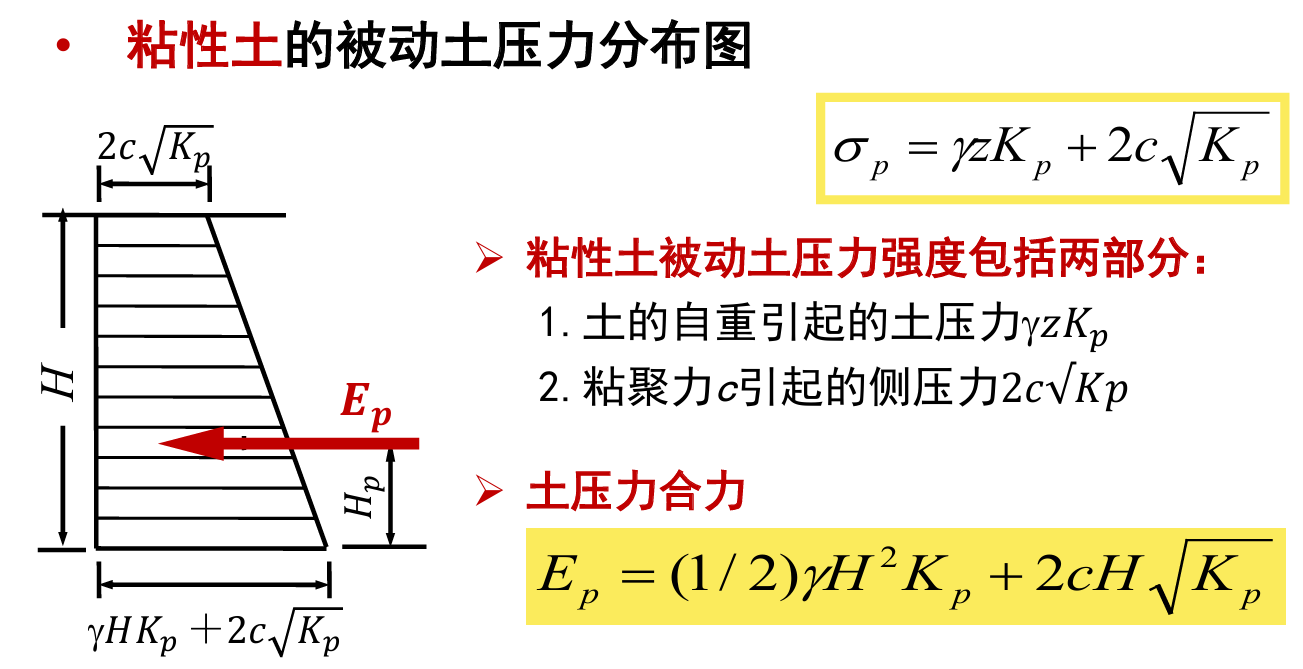
\includegraphics[width=0.8\textwidth]{../figure/beidong.png}
    \caption{被动土压力}
\end{figure}

于是,对于粘性土,我们采用流体力学里面一样的推导过程,被动土压力就是一个矩形+一个三角形,太简单了:

$$
E_p = \frac{1}{2} K_p \gamma H^2 + 2c \sqrt{K_p} H
$$
对于主动土压力,是一个改变的三角形,也很简单:
$$
E_a = \frac{1}{2} K_a \gamma H'^2,H' = H - \frac{2c}{\gamma \sqrt{K_a}}
$$

\end{example}

\begin{example}
    简单叙述下波浪荷载生成的几个阶段,波浪荷载的破坏力和什么相关,如何应对波浪荷载?

    波浪荷载的生成包括三个阶段:
    \begin{enumerate}
        \item 深水区($d > \frac{L}{2}$):海底的摩擦阻力影响较小,波浪平稳传播,称为深水推进波。
        \item 浅水区($d < \frac{L}{2}$):海底的摩擦阻力影响较大,波浪高度增加,波长减小,波陡相应增大,称为浅水推进波。
        \item 近岸区($d < \frac{L}{20}$):波浪高度达到极限,波浪破碎,形成波浪破碎带。
        \item 破碎后重新形成波浪,最终演变为击岸波。
    \end{enumerate}

    影响因素包括波浪特性、构筑物型式(圆柱体上的波浪荷载与直径波长比有关)、地形地貌、海底坡度等。    

    可以安装调谐液体阻尼器(Tuned Liquid Damper, TLD)是一种固定在结构上的半充满液体的水箱,属于被动控制装置中的吸振器减振体系。它主要利用水箱中液体的晃动和部分耗能来减轻结构的振动反应。
\end{example}

\begin{example}
    叙述土的冻胀原理

    冻胀原理:水体向冻结锋面迁移,使在冻结面上形成了冰夹层和冰透镜体,导致冻层膨胀,地层隆起。同时土体冻结时,土颗粒之间相互隔离,产生位移,使土体积产生不均匀膨胀。

\end{example}

\begin{example}
    我国现行《建筑结构荷载规范》GB50009-2012在确定风荷载时,规定了
A、B、C、D四类地貌,其中标准地貌类别为:()

基本风压由10m高度风压确定,标准地貌为B类
\end{example}

\begin{example}
    统计风速时,时距越长,公称风速最大值越大。

    公称风速是在一定时距内的平均风速,所以时距越小,公称风速最大值越大。因为短期内出现风力的平均显然大于长期风力的平均(不是时时刻刻有风的)。
\end{example}

\begin{remark}
    国家规定基本风速时距为10min
\end{remark}

\begin{example}
    在横风向共振所处区域内:(D)

    A.斯托哈数接近于常数0.2; 

    B.斯托哈数离散性很大;

    C.风漩涡脱落频率与风速成正比; 

    D.风漩涡脱落频率保持常数.
\end{example}

\begin{example}
    杭州某高层建筑所在场地为C类地貌,已知杭州基本风压 $w_0 = 0.45\,\mathrm{kN/m}^2$,$\frac{\gamma}{2g} = \frac{1}{1740}$,试分别计算该场地 $50\,\mathrm{m}$ 处的风压及对应的风速值。

    \begin{figure}[H]
        \centering
        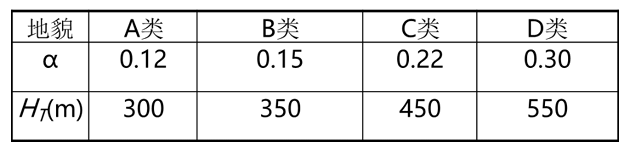
\includegraphics[width=0.5\textwidth]{../figure/3.png}
        \caption{地貌参数}
    \end{figure}

    死记硬背下公式,当然可以现场推导下:
    \[
    w_{0c} = w_{0s} \left( \frac{H_{Ts}}{z_s} \right)^{2\alpha_s} \left( \frac{H_{Tc}}{z_c} \right)^{-2\alpha_c}=0.45 \left( \frac{350}{10} \right)^{2 \times 0.15} \left( \frac{450}{10} \right)^{-2 \times 0.22} = 0.245 \,\mathrm{kN/m}^2
    \]
    于是,求得未知地区的标准风压后,计算其50m高度的风压:
    \[
    w_c = w_{0c} (\frac{50}{10})^{2 \times 0.22}=0.497\,\mathrm{kN/m}^2
    \]
    计算风速:
    \[
    w_c = \frac{1}{2} \rho v^2 = \frac{1}{2} \frac{\gamma}{g} v^2
    \]
    \[
    v = \sqrt{2 w_c g / \gamma} = \sqrt{0.497  / (1/1740)} = 29.4\,\mathrm{m/s}
    \]
\end{example}

\begin{example}
    已知:某矩形高层建筑,结构高度 $H=40\,\mathrm{m}$,平面长度 $D=30\,\mathrm{m}$,宽度 $B=25\,\mathrm{m}$,建造于城市市郊,地面粗糙度 $\alpha_a=0.22$,标准地貌的地面粗糙指数 $\alpha_s=0.15$,基本风压 $w_0=0.5\,\mathrm{kN/m}^2$。假设不考虑脉动风影响,沿高度均匀分成四段进行近似计算。求:顺风向风产生的建筑底部弯矩?

    \textbf{解:}

    1. 计算每段高度:
    \[
    \Delta h = \frac{H}{4} = \frac{40}{4} = 10\,\mathrm{m}
    \]
    各段中心高度分别为 $z_1=5\,\mathrm{m}$,$z_2=15\,\mathrm{m}$,$z_3=25\,\mathrm{m}$,$z_4=35\,\mathrm{m}$。

    2. 计算各段风压(采用风压高度变化系数):

    同时我们必须考虑截断高度,对于A、B、C、D分别是5、10、15、30m。
    \[
    w(z) = \mu_s \mu_z(z) w_0
    \]
    其中 $\mu_s = 1.3 ,\text{是体型系数},\mu_z(z)=\left( \frac{H_{Ts}}{z_s} \right)^{2\alpha_s} \left( \frac{H_{Ta}}{z_a} \right)^{-2\alpha_a} \left( \frac{z}{z_s} \right)^{2\alpha_a} = 0.54 \times (\frac{z}{z_s})^{2 \times 0.22}$
    \begin{align*}
    w_1 &= 1.3 \times 0.54 \times (15/10)^{0.44} \times 0.5 = 0.42\,\mathrm{kN/m}^2 \\
    w_2 &= 1.3 \times 0.54 \times (15/10)^{0.44} \times 0.5 = 0.42\,\mathrm{kN/m}^2 \\
    w_3 &= 1.3 \times 0.54 \times (25/10)^{0.44} \times 0.5 = 0.52\,\mathrm{kN/m}^2 \\
    w_4 &= 1.3 \times 0.54 \times (35/10)^{0.44} \times 0.5 = 0.61\,\mathrm{kN/m}^2 \\
    \end{align*}
    3. 计算各段风荷载(作用面积 $A = B \times \Delta h = 25 \times 10 = 250\,\mathrm{m}^2$):
    \[
    F_i = w_i \cdot B \cdot \Delta h
    \]

    \begin{align*}
    F_1 &= 0.42 \times 250 = 105\,\mathrm{kN} \\
    F_2 &= 0.42 \times 250 = 105\,\mathrm{kN} \\
    F_3 &= 0.52 \times 250 = 130\,\mathrm{kN} \\
    F_4 &= 0.61 \times 250 = 152.5\,\mathrm{kN} \\
    \end{align*}
    4. 计算各段力臂(至底部距离):
    \begin{align*}
    l_1 &= 35\,\mathrm{m} \\
    l_2 &= 25\,\mathrm{m} \\
    l_3 &= 15\,\mathrm{m} \\
    l_4 &= 5\,\mathrm{m} \\
    \end{align*}

    5. 计算底部弯矩:
    \[
    M = \sum_{i=1}^{4} F_i \cdot l_i = 105 \times 35 + 105 \times 25 + 130 \times 15 + 152.5 \times 5
    \]
    \[
    = 3675 + 2625 + 1950 + 762.5 = 10512.5\,\mathrm{kN \cdot m}
    \]

    \textbf{答:} 顺风向风产生的建筑底部弯矩约为 $10512.5\,\mathrm{kN \cdot m}$。

\end{example}

\begin{example}
    什么情况下要考虑结构横风向风振效应?如何进行横风向风振验算?什么情况下要考虑结构横风向风振效应?如何进行横风向风振验算?

    当横向风作用引起结构共振时,结构横风向风振效应不可忽略。通过雷诺数验算。
\end{example}



\begin{example}
已知一伸臂梁如图 9-12 所示。梁所能承担的极限弯矩为 \( M_u \),若梁内弯矩 \( M > M_u \) 时,梁便失效。现已知各变量均服从正态分布,其各自的平均值及标准差为:荷载统计参数:\( \mu_p = 4 \text{kN} \),\( \sigma_p = 0.8 \text{kN} \);跨度统计参数:
\[
\mu_l = 6 \text{m}, \sigma_l = 0.1 \text{m} \text{;极限弯矩统计参数:} \mu_{M_u} = 20 \text{kN} \cdot \text{m}, \sigma_{M_u} = 2 \text{kN} \cdot \text{m} \text{。}
\]
试用中心点法计算该构件的可靠指标 \( \beta \)。

\begin{figure}[H]
\centering
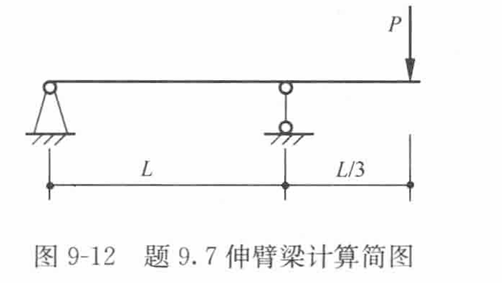
\includegraphics[width=0.6\textwidth]{../figure/5.png}
\end{figure}

\[
Z = M_u - \frac{1}{3} P l
\]
\[
\begin{cases}
F_1 + F_2 = P \\
F_1 l + P \cdot \frac{l}{3} = 0
\end{cases}
\]
\[
F_1 = -\frac{1}{3} P, \quad F_2 = \frac{4}{3} P
\]
\[
\mu_Z = \mu_{Mu} - \frac{1}{3} \mu_P \mu_l = 20 - \frac{1}{3} \times 4 \times 6 = 12 \text{ kN} \cdot \text{m}
\]
偏导数计算:
\[
\frac{\partial Z}{\partial M_u} = 1, \quad \frac{\partial Z}{\partial P} =-\frac{1}{3} l, \quad \frac{\partial Z}{\partial l} = -\frac{1}{3} P
\]
标准差计算:
\[
\sigma_Z = \sqrt{
    (\sigma_{M_u})^2 + \left(\frac{1}{3} \mu_l \sigma_ P \right)^2 + \left(\frac{1}{3} \mu_P \sigma_l \right)^2
} 
= 2.56
\]
计算系数 $\beta$:
\[
\beta = \frac{\sigma_Z}{M_Z} = \frac{2.56}{12} = 0.213
\]
\end{example}

\ifx\allfiles\undefined
\end{document}
\fi